\documentclass[a4paper, 12pt]{article}
\newcommand{\template}{../../Templates}
\usepackage{\template/package}
\usepackage{caption}
\usepackage{tikz}
\usepackage{xcolor}
\usepackage{pgfplots}
\usepackage{longtable}

\definecolor{colore1}{RGB}{70,188,198}
\definecolor{colore2}{RGB}{66,134,245}
\definecolor{colore3}{RGB}{234,66,53}
\definecolor{colore4}{RGB}{250,189,3}
\definecolor{colore5}{RGB}{147, 112, 219}
\definecolor{colore6}{RGB}{0,128,0}
\graphicspath{{../../Assets}}

\newcommand{\Titolo}{Specifiche tecniche}
\newcommand{\Data}{30/03/2024}
\newcommand{\Versione}{0.2.0}
\newcommand{\Descrizione}{Descrizione delle scelte architetturali e di design del progetto}
\newcommand{\Stato}{Non approvato}
\newcommand{\Verificatori}{/}
\newcommand{\Destinatari}{prof. Tullio Vardanega \\ & prof. Riccardo Cardin}
\newcommand{\Redattori}{Carlo Rosso}
\newcommand{\Approvatori}{/}
\raggedright

\newcommand{\Gruppo}{SWEnergy}
\newcommand{\Mail}{\href{mailto:project.swenergy@gmail.com}{project.swenergy@gmail.com}}

\renewcommand\familydefault{\sfdefault} % Set default font family to sans-serif
\linespread{1.5}

\hypersetup{
	pdfmenubar=true,            % show Acrobat’s menu?
	pdfstartview={FitH},        % fits the width of the page to the window
	colorlinks=true,            % false: boxed links; true: colored links
	linkcolor=black,            % color of internal links (change box color with linkbordercolor)
	% citecolor=green,          % color of links to bibliography
	% filecolor=magenta,        % color of file links
	urlcolor=[RGB]{156,1,198}   % color of external links
}

\newcommand{\copertina}{
	\begin{titlepage}
		\vspace*{-3.5cm}
		\makebox[\textwidth]{
\includegraphics[width=\paperwidth]{header.png}}
		\begin{center}
			
\includegraphics[width=1\textwidth]{logo.png}	\\
			\vspace{1cm}
			\Mail	\\
			\vspace{0.5cm}
			\textbf{\begin{LARGE} \Titolo \end{LARGE}}		\\
			\vspace{1cm}
			\textbf{Descrizione:} \Descrizione{}			\\
			\vspace{1cm}
			\begin{tabular}{ll}
				\textbf{Stato}               & \Stato              \\
				\textbf{Data}                & \Data               \\
				\midrule
				\textbf{Redattori}           & \Redattori          \\
				\textbf{Verificatori}        & \Verificatori       \\

				\ifdefined\Approvatori
				\textbf{Approvatori}         & \Approvatori        \\
				\fi

				\ifdefined\ApprovatoriInterni
				\textbf{Approvatori interni} & \ApprovatoriInterni \\
				\fi

				\ifdefined\ApprovatoriEsterni
				\textbf{Approvatori esterni} & \ApprovatoriEsterni \\
				\fi

				\ifdefined\Destinatari
				\textbf{Destinatari}         & \Destinatari        \\
				\fi

				\midrule

				\ifdefined\Versione
				\textbf{Versione}            & \Versione           \\
				\fi
			\end{tabular}
		\end{center}
		\vspace{4cm}
	\end{titlepage}
	\newpage
}

\fancypagestyle{plain}{
	\fancyhf{}
	\rhead{ 
\includegraphics[scale=0.05]{horizontal_logo.png}}
	\lhead{\Titolo \ifdefined\Versione \ \Versione \fi}
	%\lfoot{\Titolo}
	\rfoot{\thepage{} di \pageref{LastPage}}
	\renewcommand{\headrulewidth}{0.2pt}
	\renewcommand{\footrulewidth}{0.2pt}
}
\pagestyle{plain}


\begin{document}

\copertina{}
\section*{Registro delle modifiche}
 {
  \scriptsize
  \begin{tabular}{p{0.10\linewidth}p{0.10\linewidth}p{0.15\linewidth}p{0.15\linewidth}p{0.15\linewidth}p{0.19\linewidth}}
	  \textbf{Versione} & \textbf{Data} & \textbf{Redattore}     & \textbf{Verificatore} & \textbf{Approvatore} & \textbf{Descrizione}                                                                                                                     \\
	  \toprule
	  2.0.1             & 27/02/2024    & Davide Maffei          & Carlo Rosso           & /                    & Correzioni in seguito alla revisione RTB                                                                                                 \\
	  \hline
	  2.0.0             & 27/02/2024    & /                      & /                     & Niccolò Carlesso     & Approvazione finale del documento                                                                                                        \\
	  \hline
	  1.5.0             & 26/02/2024    & Alessandro Tigani Sava & Carlo Rosso           & /                    & Descrizione metriche di qualità                                                                                                          \\
	  \hline
	  1.4.1             & 14/02/2024    & Davide Maffei          & Giacomo Gualato       & /                    & Allineamento delle sezioni dei ruoli                                                                                                     \\
	  \hline
	  1.4.0             & 14/02/2024    & Davide Maffei          & Giacomo Gualato       & /                    & Creazione delle sezioni dei processi primari, di supporto e organizzativi                                                                \\
	  \hline
	  1.3.0             & 8/01/2024     & Carlo Rosso            & Niccolò Carlesso      & /                    & Correzione della sotto-sezione "Aggiornamento delle "Norme di Progetto"" e aggiunte le sotto-sezioni "Revisione del codice" e "Codifica" \\
	  \hline
	  1.2.0             & 31/12/2023    & Carlo Rosso            & Niccolò Carlesso      & /                    & Ristrutturazione del documento per ruolo, piuttosto che per argomento                                                                    \\
	  \hline
	  1.1.0             & 30/10/2023    & Carlo Rosso            & Giacomo Gualato       & /                    & Aggiornamento della sezione dedicata alla documentazione e aggiunta una sezione dedicata agli appunti                                    \\
	  \hline
	  1.0.0             & 30/10/2023    & /                      & /                     & Giacomo Gualato      & Approvazione finale del documento                                                                                                        \\
	  \hline
	  0.2.1             & 29/10/2023    & Alessandro Tigani Sava & Niccolò Carlesso      & /                    & Modifica procedure in sezione Approvazione di un documento                                                                               \\
	  \hline
	  0.2.0             & 24/10/2023    & Matteo Bando           & Niccolò Carlesso      & /                    & Redazione sezioni Versionamento, Verifica di un documento, Approvazione di un documento                                                  \\
	  \hline
	  0.1.0             & 23/10/2023    & Alessandro Tigani Sava & Matteo Bando          & /                    & Redazione sezioni Introduzione, Strumenti, Creazione e modifica di un documento, Ruoli, Registro delle modifiche                         \\
	  \hline
  \end{tabular}
 }

\newpage
\tableofcontents
\newpage
\section{Introduzione}

Il presente documento, intitolato "Piano di Progetto", descrive e spiegare le
decisioni organizzative adottate dal gruppo SWEnergy per lo sviluppo del
progetto "\textit{Easy Meal}", proposto dall'azienda
\href{https://imolainformatica.it/}{Imola Informatica}. Il "Piano di Progetto" è
suddiviso nelle seguenti sezioni:

\begin{itemize}
	\item \textbf{Analisi dei rischi}: identifica i rischi individuati dal
	      gruppo e le strategie per mitigarli;

	\item \textbf{Modello di sviluppo}: descrive l'organizzazione temporale del
	      team di SWEnergy;

	\item \textbf{Pianificazione}: dettaglia la pianificazione del lavoro del
	      gruppo, incluse le attività, le risorse e i tempi necessari per lo
	      sviluppo del progetto;

	\item \textbf{Preventivo}: presenta il preventivo delle ore di lavoro e il
	      costo totale del progetto;

	\item \textbf{Consuntivo}: riporta le ore di lavoro e il costo effettivo del
	      progetto fino al momento della stesura del piano di progetto della
	      fase corrente: RTB.
\end{itemize}

\subsection{Scopo del documento}

Questo documento ha lo scopo di raccogliere in modo organico, coerente e
uniforme tutte le informazioni riguardanti la pianificazione del progetto, al
fine di fornire un riferimento per la gestione dello stesso. Al termine della
prima fase del progetto (RTB), verrà utilizzato per valutare l'andamento del
lavoro e per spiegare le decisioni adottate durante la pianificazione.

\subsection{Scopo del prodotto}

"\textit{Easy Meal}" è una web app progettata per gestire le prenotazioni
presso i ristoranti, sia dal lato dei clienti che dei ristoratori. Il prodotto
finale sarà composto da due parti:

\begin{itemize}
	\item \textbf{Cliente}: consente ai clienti di prenotare un tavolo presso un
	      ristorante, visualizzare il menù e effettuare un ordine;

	\item \textbf{Ristoratore}: consente ai ristoratori di gestire le
	      prenotazioni e gli ordini dei clienti, oltre a visualizzare la lista
	      degli ingredienti necessari per preparare i piatti ordinati.
\end{itemize}

\subsection{Glossario}

Al fine di evitare ambiguità linguistiche e garantire un'utilizzazione coerente
delle terminologie nei documenti, il gruppo ha redatto un documento interno
chiamato "Glossario". Questo documento definisce in modo chiaro e preciso i
termini che potrebbero generare ambiguità o incomprensione nel testo. I termini
presenti nel Glossario sono identificati da una 'G' (per esempio parola$_G$) a
pedice.

\subsection{Riferimenti}

\subsubsection{Normativi}
\begin{itemize}
	\item "\textit{Way of Working}";
	\item 	\href{https://www.math.unipd.it/~tullio/IS-1/2023/Progetto/C3.pdf}
	      {Documento del capitolato d'appalto C3 - \textit{Easy Meal}};
	\item \href{https://www.math.unipd.it/~tullio/IS-1/2023/Dispense/PD2.pdf}
	      {Regolamento del progetto};
\end{itemize}

\subsubsection{Informativi}

Slide dell'insegnamento di Ingegneria del Software:
\begin{itemize}
	\item \href{https://www.math.unipd.it/~tullio/IS-1/2023/Dispense/T3.pdf}
	      {Modelli di sviluppo del software};
	\item \href{https://www.math.unipd.it/~tullio/IS-1/2023/Dispense/T4.pdf}
	      {Gestione di progetto};
	\item \href{https://www.math.unipd.it/~tullio/IS-1/2023/Dispense/T5.pdf}
	      {Analisi dei requisiti};
\end{itemize}

\subsection{Scadenze}
Il \textit{team} di SWEnergy si impegna a rispettare le seguenti scadenze per il
completamento del progetto:
\begin{itemize}
	\item \textbf{Prima revisione (avanzamento RTB}: 21 dicembre 2023;
	\item \textbf{Seconda revisione (avanzamento PB)}: da definire;
	\item \textbf{Terza revisione (avanzamento CA)}: da definire;
\end{itemize}

\section{Tecnologie adottate}

\subsection{Tecnologie per la codifica}

\subsection{Tecnologie per l'analisi statica del codice}

\subsection{Tecnologie per l'analisi dinamica del codice}

% qui sono ci mettiamo la tabella riassuntiva

\section{Architettura}

Approfondiamo l'architettura scelta per Easy-Meal, spiegando le scelte
architetturali e i \textit{pattern} utilizzati per lo sviluppo dell'applicazione partendo
dalla struttura generale del sistema e passando poi ai dettagli implementativi.

\subsection{Architettura di Deployment}

SWEnergy ha deciso di adottare un'architettura monolitica a tre livelli (\textit{3-tier
architecture}) per implementare Easy-Meal. 
Questa scelta è stata determinata dalla necessità di costruire una 
\textit{web application} che permetta agli utenti di accedere al sistema da qualsiasi 
dispositivo connesso a Internet. L'architettura a tre livelli
separa la logica di presentazione dalla logica di \textit{business} e dal \textit{database}.
I livelli comunicano tra loro attraverso interfacce ben definite, in particolare:
\begin{itemize}
	\item \textbf{Livello di Presentazione (\textit{Frontend})}: rappresentato da Angular, riceve i dati dall'utente e visualizza i risultati restituiti dal \textit{backend}.
	\item \textbf{Livello di Logica Applicativa (\textit{Backend})}: rappresentato da NestJS. Gestisce la logica di \textit{business}, elabora le richieste provenienti dal \textit{frontend} e interagisce con il \textit{database} per recuperare o salvare i dati.
	\item \textbf{Livello di Dati (\textit{Database})}: rappresentato dal \textit{database} PostgreSQL, si occupa della gestione dei dati.
\end{itemize}

Questo approccio ha permesso al team di sviluppo di lavorare in modo parallelo 
sul \textit{frontend} e sul \textit{backend}, riducendo i tempi di sviluppo e 
facilitando il \textit{testing} del sistema. Inoltre, offre la possibilità di scalare ciascun 
livello separatamente, in modo da garantire prestazioni ottimali e una 
maggiore flessibilità. Infine, è possibile sostituire l'implementazione di 
uno dei livelli senza dover toccare gli altri, garantendo una maggiore 
manutenibilità del sistema.
In particolare lo sviluppo di Easy-Meal è cominciato partendo dal \textit{database},
l'elemento su cui abbiamo posto maggiore enfasi, in quanto è il cuore del
sistema. Successivamente sono stati sviluppati il \textit{backend} e il
\textit{frontend}, in modo da garantire una corretta integrazione tra i
diversi livelli dell'applicazione. SWEnergy ha deciso di utilizzare questa
metodologia, perché le funzionalità messe a disposizione da Easy-Meal al livello
della logica di \textit{business} sono principalmente delle semplici operazioni CRUD, che non richiedono
un'interazione complessa tra i diversi livelli dell'applicazione.

\subsection{Pattern Architetturali}

Easy-Meal è stato sviluppato utilizzando due \textit{pattern} architetturali:
Model-View-Controller e Dependency Injection. Infatti, SWEnergy ha scelto di
adottare Angular e NestJS, due \textit{framework} che implementano questi \textit{pattern} in modo
nativo, garantendo una struttura ben definita e una maggiore manutenibilità del
codice.

\subsubsection{Model-View-Controller}

Il \textit{pattern} architetturale Model-View-Controller (MVC) è stato utilizzato per
suddividere le responsabilità tra i diversi componenti dell'applicazione. In
particolare, il \textit{model} rappresenta i dati dell'applicazione e fornisce i
metodi di accesso e di modifica di tali dati. NestJS è il \textit{framework} che
implementa il \textit{backend} nell'applicativo e fornisce le API\g di accesso ai dati
di modifica tramite i \textit{controller}. Angular, invece, è il \textit{framework} che
implementa il \textit{frontend} e fornisce le interfacce grafiche per la gestione delle
interazione con l'utente, ovvero la \textit{view}. I \textit{component} e i
\textit{controller} sono responsabili di gestire le interazioni tra la 
\textit{view} e il \textit{model},
aggiornando i dati in base alle azioni dell'utente. L'aggiornamento della
visualizzazione dei dati è gestito da Angular, che attraverso il \textit{data
binding} permette di mantenere sincronizzati i dati presenti nel \textit{model}
con la \textit{view}.

\subsubsection{Dependency Injection}

Il \textit{pattern} Dependency Injection (DI) è stato utilizzato per gestire le
dipendenze tra i diversi componenti dell'applicazione. In particolare, Angular
utilizza la DI per iniettare i servizi all'interno dei componenti, permettendo
di scrivere codice più modulare e manutenibile. NestJS, invece, utilizza la DI
per iniettare i servizi all'interno dei \textit{controller}, permettendo di separare la
logica di \textit{business} dalla logica di accesso ai dati. Questo approccio consente di
creare componenti indipendenti e riutilizzabili, facilitando la manutenibilità
dell'applicazione. Infine la divisione in moduli rende il codice facilmente
testabile, in quanto è possibile sostituire i servizi con dei \textit{mock} per
testare i componenti in modo isolato.

\subsection{Frontend}

Di seguito sono proposti alcuni diagrammi delle classi per il \textit{frontend}
di Easy-Meal. Poiché la struttura del \textit{frontend} è piuttosto vasta, ma
ridondante, nel senso che il \textit{pattern} \textit{dependency injection} è applicato
allo stesso modo per tutti i componenti, si è deciso di selezionare alcuni
esempi significativi.

\subsubsection{GenericService}

\begin{figure}[H]
	\centering
	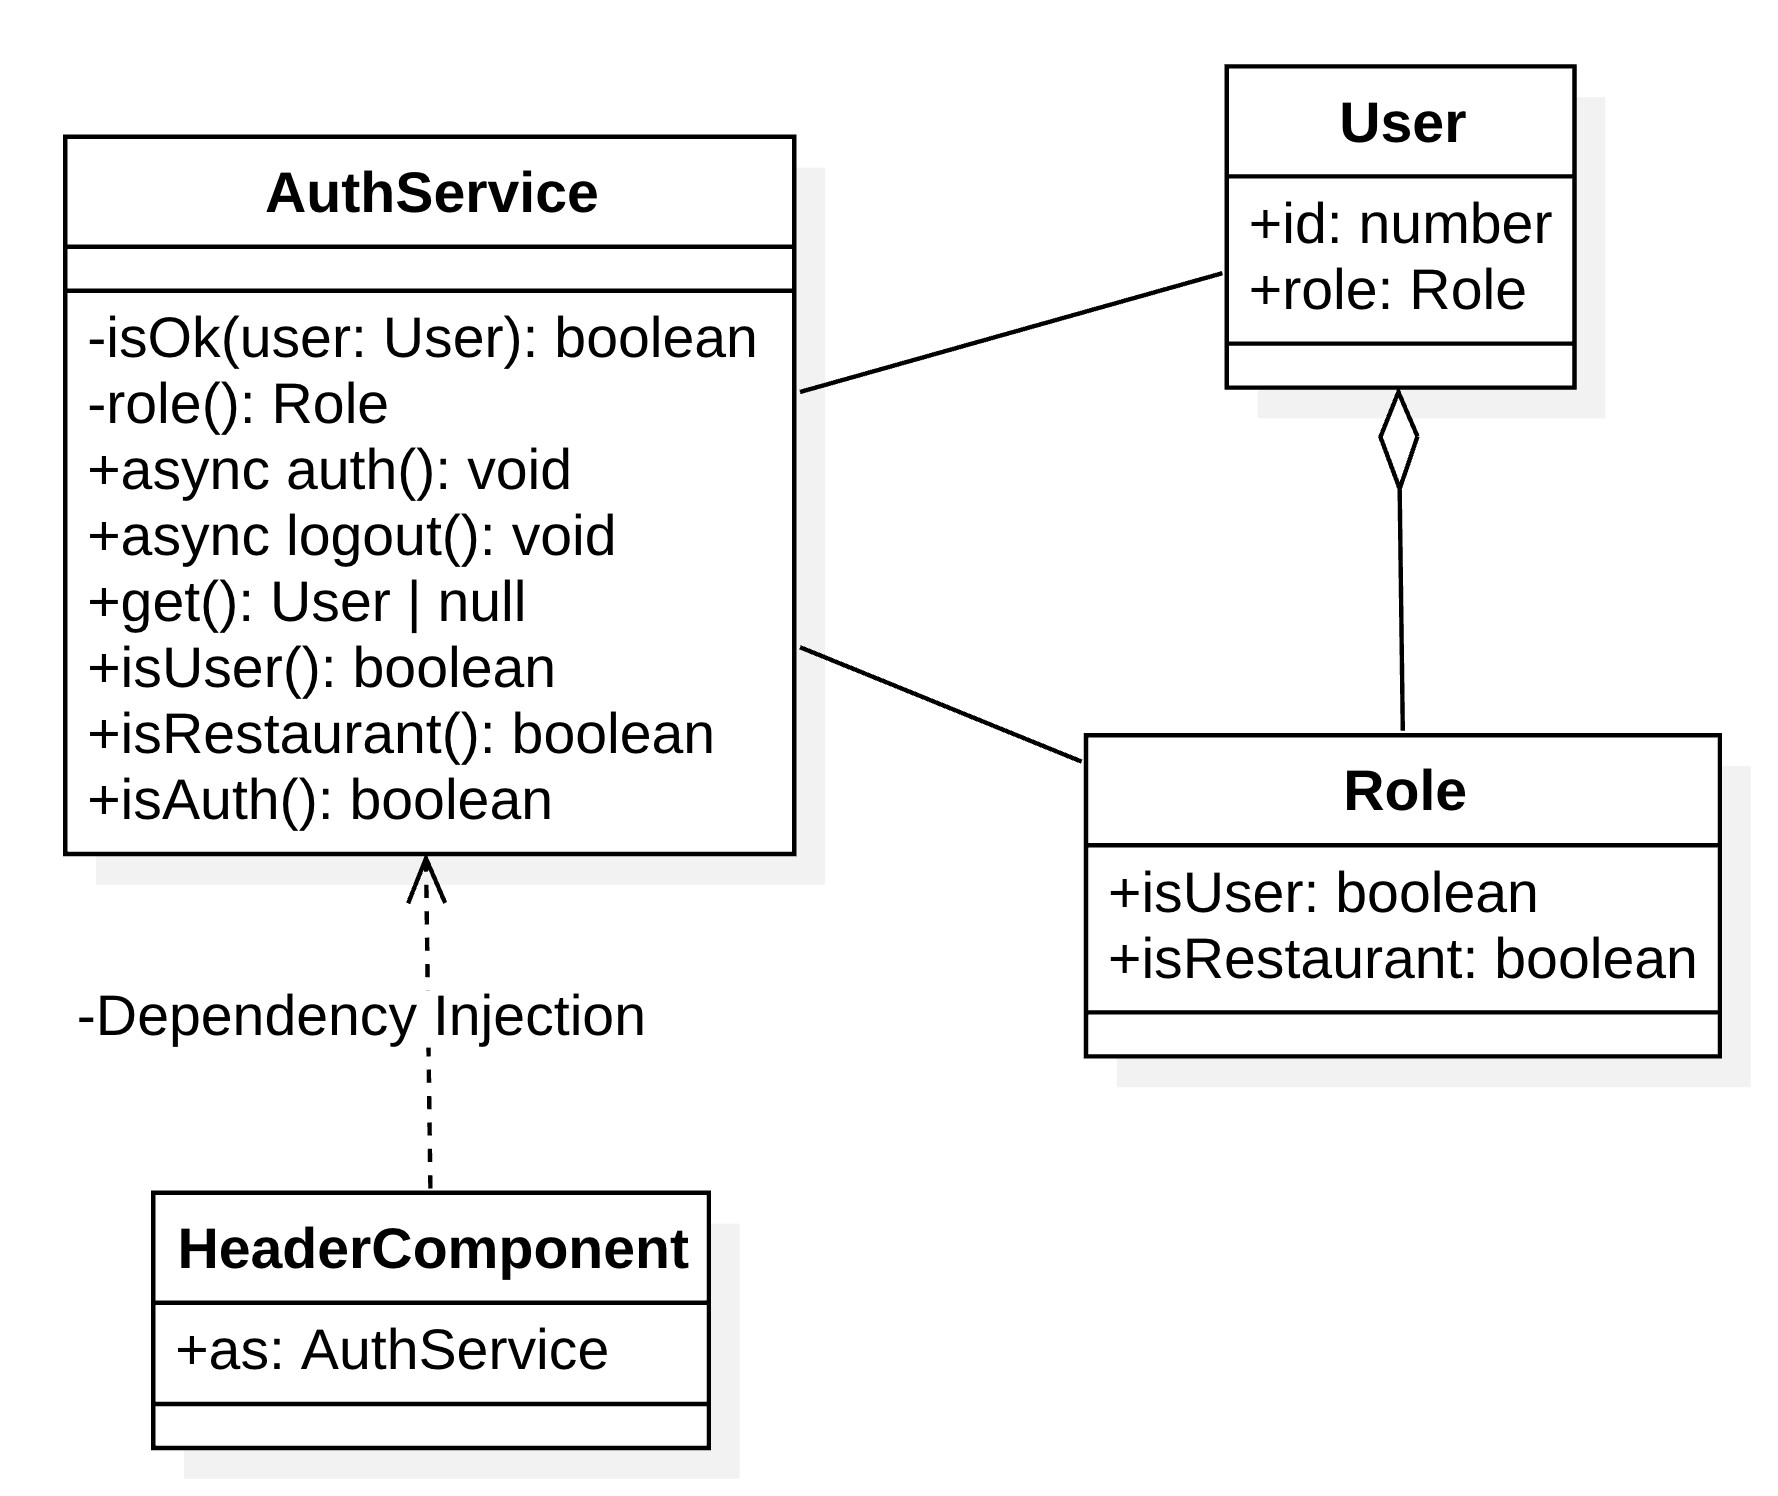
\includegraphics[width=0.5\textwidth]{PB/specifiche-tecniche/auth-service.png}
	\caption{Diagramma delle classi per AuthService}
\end{figure}

In questo caso, viene mostrato come viene iniettato un servizio all'interno di
un componente. Lo \textit{specimen} scelto è il servizio AuthService,
che è responsabile della gestione dell'autenticazione dell'utente. Iniettando
AuthService all'interno del componente HeaderComponent, i metodi pubblici
definiti in AuthService possono essere utilizzati per gestire l'autenticazione
dell'utente. In particolare, HeaderComponent utilizza AuthService per gestire i
\textit{link} del menu di navigazione in base allo stato di autenticazione e al ruolo 
dell'utente. In questo modo viene favorita la separazione delle responsabilità
e la modularità del codice, rendendo il componente HeaderComponent più
manutenibile e permettendo di riutilizzare AuthService in altri componenti.

\subsubsection{MessageService}

\begin{figure}[H]
	\centering
	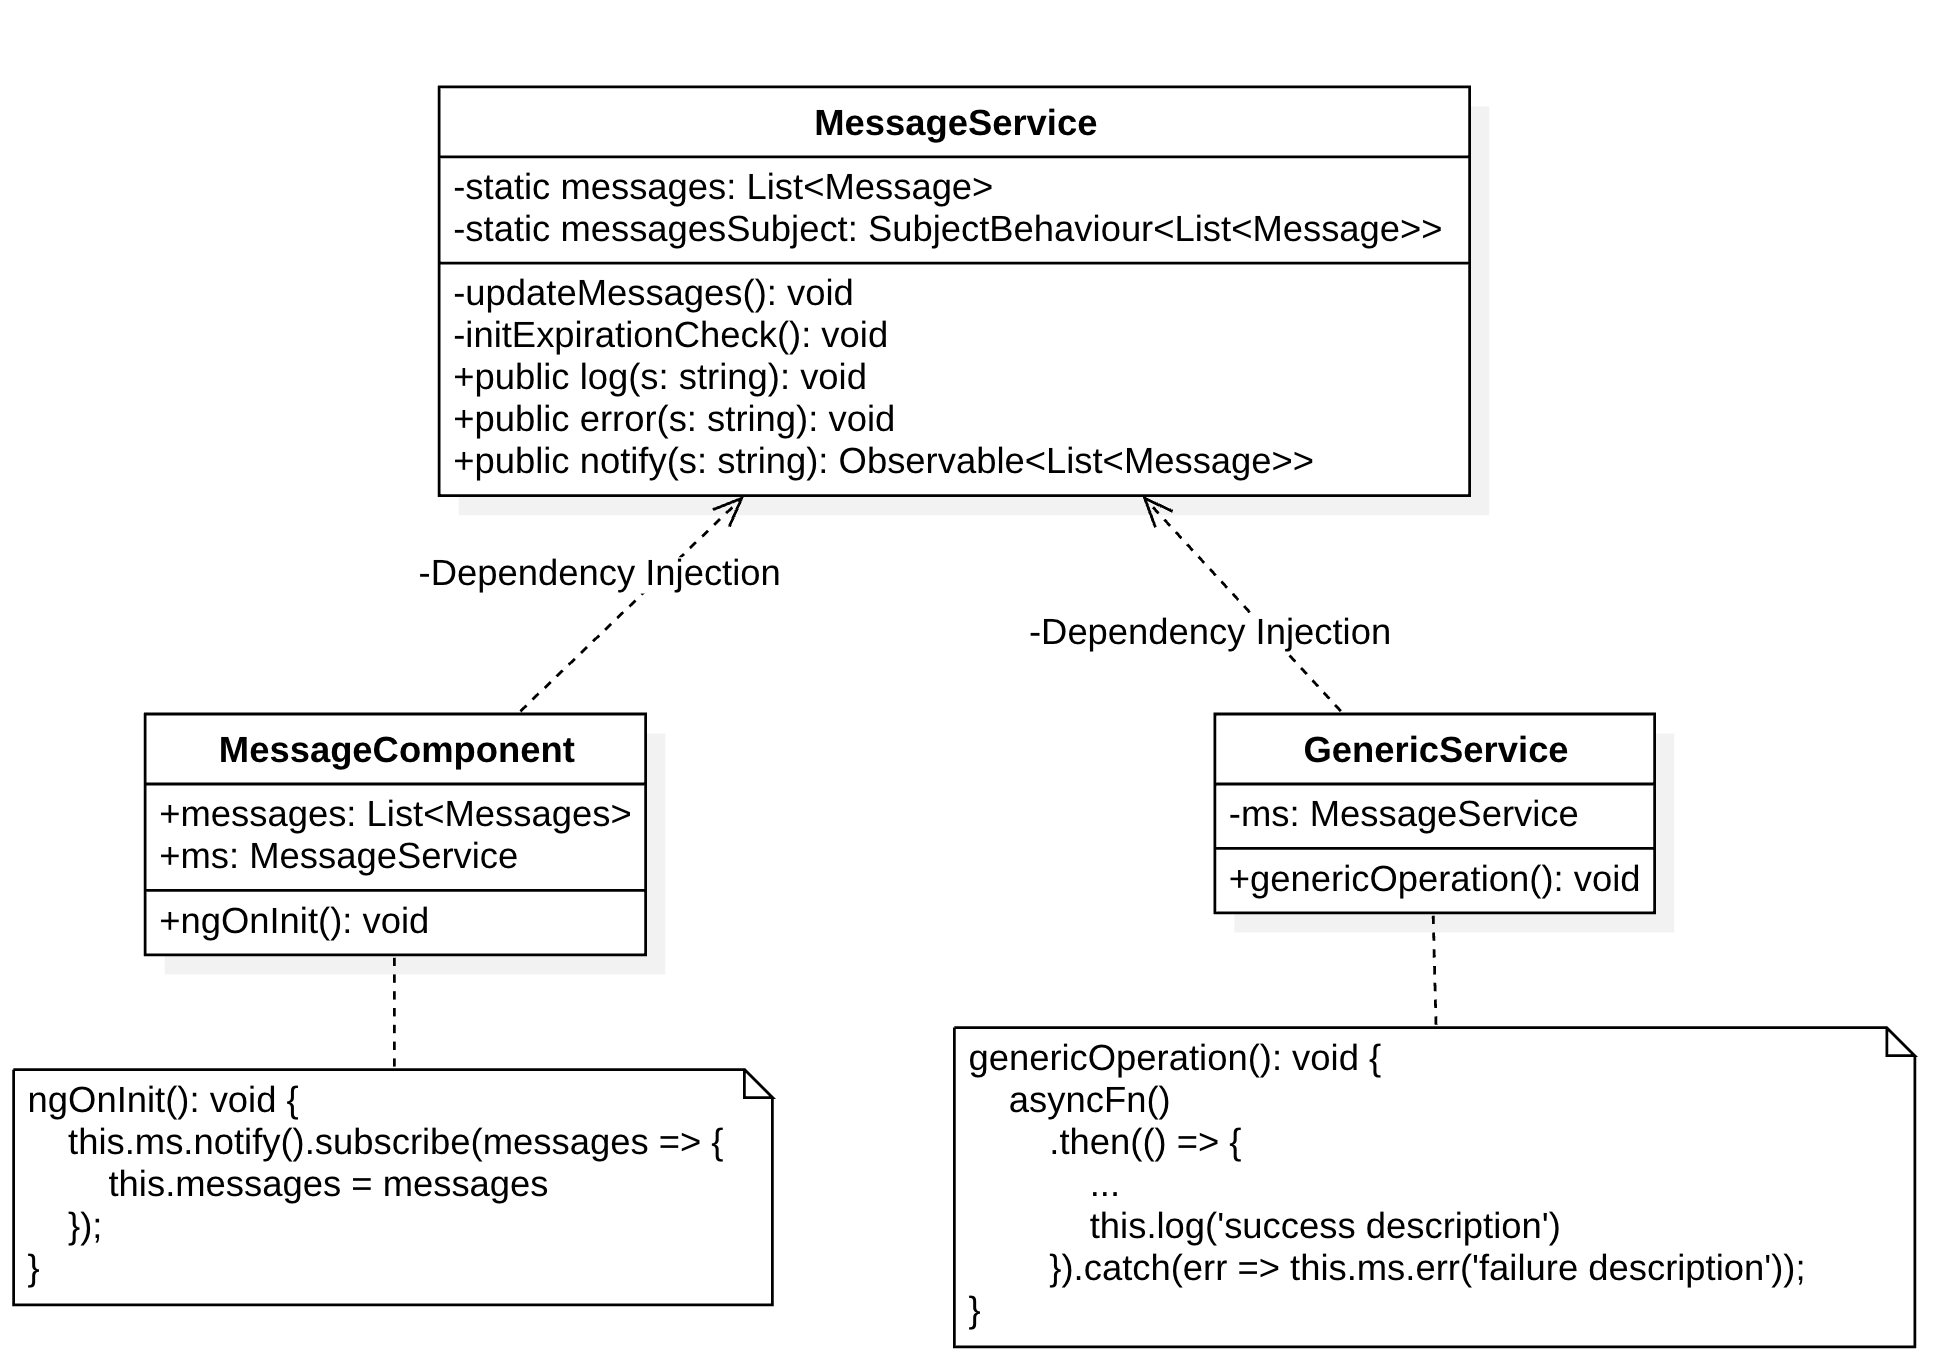
\includegraphics[width=0.8\textwidth]{PB/specifiche-tecniche/message-service.png}
	\caption{Diagramma delle classi per il MessageService}
\end{figure}

La \textit{dependency injection} (DI) in Angular è un \textit{design pattern} che 
consente di fornire dipendenze alle classi in modo automatizzato. In questo 
caso, la classe MessageService viene iniettata sia nella classe 
MessageComponent che nella classe GenericService.
Questo è reso possibile dichiarando MessageService come dipendenza nei 
costruttori delle rispettive classi.
L'annotazione \texttt{@Injectable} viene utilizzata sulla classe MessageService 
per indicare che questa può essere iniettata come dipendenza.\\
MessageService è implementato come \textit{singleton} in Angular. Un \textit{singleton} garantisce 
che una sola istanza della classe venga creata e condivisa in tutta 
l'applicazione.
Questo è importante per la gestione centralizzata dello stato e delle operazioni 
comuni, come la gestione dei messaggi.
In Angular, il \textit{pattern singleton} è implicitamente implementato tramite il 
sistema DI, poiché il servizio è registrato nel \textit{root injector}, 
garantendo una singola istanza.\\
Angular offre un potente meccanismo di \textit{data binding} che consente alla 
vista di aggiornarsi automaticamente quando i dati del modello cambiano.
Nella classe MessageComponent, il metodo \texttt{ngOnInit} utilizza 
l'osservabile restituito da ms.notify() per iscriversi agli aggiornamenti dei 
messaggi.
Quando i messaggi vengono aggiornati nel MessageService, la vista associata a 
MessageComponent si aggiorna automaticamente per riflettere i nuovi dati.
Questo è facilitato dall'utilizzo di Subject o BehaviorSubject in 
MessageService, che emettono nuovi valori quando i messaggi cambiano.\\
In sostanza, in questo modo si utilizza un servizio per condividere dati tra
componenti che non hanno una relazione gerarchica.



\subsection{Backend}
Il \textit{backend} dell'applicazione è stato realizzato utilizzando NestJS, il quale sfrutta diversi \textit{pattern} creazionali, strutturali ed architetturali.

\subsubsection{Dependency Injection}
Gestisce la creazione delle dipendenze. 
NestJS integra nativamente un sistema di \textit{Dependency Injection} che semplifica l'iniezione delle dipendenze tra i vari componenti dell'applicazione. 
Utilizza il concetto di \textit{provider} per registrare e risolvere le dipendenze.
Un esempio di utilizzo è la registrazione e l'iniezione di servizi nei moduli, generalmente eseguita come nel codice di esempio sottostante.
\begin{lstlisting}
	import { Injectable } from '@nestjs/common';

	@Injectable()
	export class UsersService { // Implementation }
	
	import { Module } from '@nestjs/common';
	import { UsersService } from './users.service';
	
	@Module({
	  providers: [UsersService],
	  exports: [UsersService],
	})
	export class UsersModule {}
\end{lstlisting}
I vantaggi nell'utilizzo della Dependency Injection sono:
\begin{itemize}
	\item \textbf{Separazione delle Preoccupazioni}: migliora la modularità e la manutenibilità del codice.
	\item \textbf{Riusabilità del Codice}: i componenti possono essere riutilizzati in diverse parti dell'applicazione senza dover gestire manualmente le loro dipendenze.
	\item \textbf{Testabilità}: semplifica il \textit{testing} unitario poiché consente di sostituire facilmente le dipendenze con versioni \textit{mock} durante i test.
	\item \textbf{Flessibilità e Scalabilità}: consente di sostituire o estendere facilmente le dipendenze senza modificare il codice esistente.
\end{itemize}


\subsubsection{Module Pattern}
Il codice dell'applicazione è suddiviso in moduli, ognuno dei quali incapsula una funzionalità specifica. 
I moduli possono importare altri moduli, rendendo l'applicazione altamente modulare e facilmente manutenibile.
Ogni modulo può contenere \textit{controller}, servizi, \textit{provider} e altre risorse.
I moduli in NestJS sono definiti usando il decoratore "Module", che specifica i componenti che fanno parte del modulo e le loro dipendenze.
\begin{lstlisting}
	import { Module } from '@nestjs/common';
	import { UsersService } from './users.service';
	import { UsersController } from './users.controller';
	
	@Module({
	  providers: [UsersService],
	  controllers: [UsersController],
	})
	export class UsersModule {}
\end{lstlisting}
I vantaggi dell'utilizzo del \textit{Module Pattern} includono:
\begin{itemize}
	\item \textbf{Organizzazione del Codice}: aiuta a mantenere il codice ben organizzato, rendendo più facile trovare e gestire le parti dell'applicazione.
	\item \textbf{Manutenibilità}: ogni modulo può essere sviluppato e manutenuto indipendentemente dagli altri.
	\item \textbf{Riusabilità}: possono essere riutilizzati in altre applicazioni o parti della stessa applicazione.
	\item \textbf{Scalabilità}: facilitando la gestione delle dipendenze e la composizione dei moduli, il Module Pattern supporta la scalabilità dell'applicazione.
\end{itemize}


\subsubsection{Controller-Service Pattern}
NestJS separa la logica di presentazione dalla logica di \textit{business}. \\
I \textit{controller} sono responsabili di gestire le richieste HTTP, mappando le richieste ai metodi appropriati e restituendo le risposte agli utenti.
Fungono da intermediari tra il \textit{client} (\textit{frontend}) e la logica di \textit{business} dell'applicazione.
Gestiscono la validazione dei parametri in ingresso e la formattazione delle risposte rilasciate.\\
I servizi contengono la logica di \textit{business} dell'applicazione. 
Sono responsabili dell'interazione con il \textit{database}, la gestione dei dati e l'implementazione delle regole di \textit{business}.
Forniscono metodi che possono essere chiamati dai \textit{controller} o da altri servizi.
Contengono operazioni CRUD, manipolazione dei dati e comunicazione con altre parti dell'applicazione.\\
Questo \textit{pattern} promuove una chiara separazione delle responabilità.
\begin{lstlisting}
	import { Controller, Get } from '@nestjs/common';
	import { UsersService } from './users.service';
	
	@Controller('users')
	export class UsersController {
	  constructor(private readonly usersService: UsersService) {}
	
	  @Get()
	  findAll() {
		return this.usersService.findAll();
	  }
	}
\end{lstlisting}
I vantaggi nell'utilizzo del \textit{Controller-Service Pattern} includono:
\begin{itemize}
	\item \textbf{Separazione delle Responsabilità}: separando la logica di presentazione (\textit{controller}) dalla logica di \textit{business (service)}, il codice diventa più modulare e facile da gestire.
	\item \textbf{Manutenibilità}: le modifiche alla logica di \textit{business} non influenzano direttamente la logica di presentazione e viceversa, rendendo il codice più manutenibile.
	\item \textbf{Testabilità}: i servizi possono essere facilmente testati in isolamento senza la necessità di simulare richieste HTTP, migliorando la copertura dei test.
	\item \textbf{Riusabilità}: la logica di \textit{business} incapsulata nei servizi può essere riutilizzata in diverse parti dell'applicazione o in altre applicazioni.
\end{itemize}


\subsubsection{Decorator Pattern}
Il Decorator Pattern è ampiamente utilizzato in NestJS per definire metadati e configurare i componenti dell'applicazione. 
I decoratori in NestJS sono funzioni che possono essere applicate a classi, metodi, proprietà o parametri per arricchirli con comportamenti aggiuntivi o configurazioni specifiche. 
Questo \textit{pattern} permette di aggiungere funzionalità in modo dichiarativo e modulare.
I decoratori più utilizzati nell'applicativo sono:
\begin{itemize}
	\item \textbf{\textit{Module}}: definisce una classe come modulo NestJS, aggregando \textit{controller, provider}, e altri moduli.
	\item \textbf{\textit{Controller}}: definisce una classe come \textit{controller} che gestisce le richieste HTTP per un determinato percorso.
	\item \textbf{\textit{Provider}}: marca una classe come un \textit{provider} (Injectable) che può essere iniettato tramite il sistema di Dependency Injection di NestJS.
	\item \textbf{Gestione delle Rotte HTTP}: associa un metodo del \textit{controller} a una specifica rotta HTTP.
	\item \textbf{Intercettori}: applica uno o più \textit{interceptor} a un metodo specifico.
	\item \textbf{Decoratori per Parametri della Rotta}: estrae parametri dalla rotta e li passa come argomenti al metodo del \textit{controller}.
	\item \textbf{Decoratori per il Corpo della Richiesta}: estrae il corpo della richiesta e lo passa come argomento al metodo del \textit{controller}.
\end{itemize}


\subsubsection{Interceptor Pattern}
Gli \textit{interceptor} in NestJS permettono di gestire il comportamento delle richieste e delle risposte in modo centralizzato. 
Possono modificare, trasformare, o loggare i dati prima che vengano inviati al \textit{client} o al \textit{server}.
In particolare ne è stato fatto uso per la gestione del caricamento delle immagini relative ai ristoranti ed ai piatti registrati dai ristoratori.
\begin{lstlisting}
	@UseInterceptors(FileFieldsInterceptor([
		{ name: 'logo', maxCount: 1 },
		{ name: 'banner_image', maxCount: 1 },
	  ]))
	  async create(
		@UploadedFiles() files: { logo?: Express.Multer.File[], banner_image?: Express.Multer.File[] }
	  ) {
		// Implementation
	  }
\end{lstlisting}

\section{Requisiti}
Questa sezione fornisce un elenco dei requisiti minimi indispensabili per l'esecuzione dell'applicazione, illustrando le caratteristiche necessarie per configurare 
correttamente l'ambiente di sviluppo del progetto.

\subsection{Requisiti di sistema}
Affinché l'installazione e l'avvio del prodotto avvengano senza problemi e per garantire un'esperienza completa e soddisfacente nell'utilizzo 
dell'applicazione, è essenziale installare i seguenti \textit{software}.

\begin{longtable}{|c|c|c|}
	\hline
	\textbf{Componente}       & \textbf{ Versione}   & \textbf{ Riferimenti per il download} \\
	\hline
     Node.js             & $ \geq  20.x.x$            &\href{https://nodejs.org/en/}{https://nodejs.org/en/}        \\
    \hline
     npm                & $ \geq 9.x.x$            &Integrato con il download di Node.js        \\
    \hline

    \caption{Tabella dei requisiti di sistema.}
\end{longtable}


\subsection{Requisiti \textit{software}}
L'applicazione è stata testata e confermata come utilizzabile sui principali \textit{browser}, per i quali sono specificate le versioni iniziali che hanno costituito 
il punto di partenza per lo sviluppo del progetto. Durante lo sviluppo, si è considerato incrementalmente l'aggiornamento alle versioni più recenti dei singoli \textit{browser}.

\begin{longtable}{|c|c|c|}
	\hline
	\textbf{Browser}       & \textbf{ Versione}    \\
	\hline
    Google Chrome             & 123                    \\
    \hline
    Arc                       & 1.26                    \\
    \hline
    Opera GX                       & 124                    \\
    \hline
    Safari                        & 17.3                    \\
    \hline
    Microsfot Edge                 & 123                      \\
    \hline

    \caption{Tabella dei requisiti \textit{software}.}
\end{longtable}


\subsection{Requisiti \textit{hardware}}
Poiché l'applicazione funziona su un \textit{browser}, non ci sono requisiti specifici definiti dal proponente, dal capitolato o dal progetto stesso. 
Quindi, i seguenti requisiti sono considerati solo come linee guida generali per l'esecuzione del prodotto creato.

\begin{longtable}{|l|p{0.8\textwidth}|}
	\hline
	\textbf{Componente}       & \textbf{ Requisito minimo}   \\
	\hline
     Processore             &  Processore a 64 bit Quad-Core 3,2 GHz      \\
    \hline
     Memoria RAM            &  4GB DDR4       \\
    \hline
    Spazio su disco         & $ \geq  126 GB$         \\
    \hline
    Connessione Internet         & Connessione \textit{Internet} stabile e veloce, in grado di supportare le esigenze di traffico dell'applicazione         \\
    \hline

    \caption{Tabella dei requisiti \textit{hardware}.}
\end{longtable}

\end{document}
